\chapter{Introduction}\label{chapter:introduction}
The capabilities and features of \gls{vr} are continually increasing, and is now capable of providing an immersive feeling. Additionally, developers and users’ interest in telepresence is growing, because it offers many possibilities for people not to be on-site. Telepresence describes the 'the perception of presence within a physically remote or simulated site' \parencite {Draper1998}. For example, as COVID-19 spreads worldwide and people have to stay at home, the need for a social life is still essential for humans but cannot be fulfilled \parencite {Berg2020}. Therefore, the need for social interaction without being in the same location as others is increasing. Another example is climate change. Travelling worldwide for tourism is becoming less popular as flying and driving emit significant levels of CO2 \parencite {Zhang2019}. Solutions such as Skype, Zoom and other video conference applications help mitigate this need, but they are not equal to personal contact \parencite {Judge2010}. Telepresence, which teleports someone to a different location without them physically moving from their current location is a new approach to solve this problem. For telepresence, \gls{vr} is an essential feature as it provides the user with an immersive view of the virtual or real environment of a different location. However, the high resolution, the high frame rates and the low latency for the \gls{vr} glasses are challenging, because the current hardware and software is not optimized \parencite{VRReady}. High resolution is necessary to achieve an immersive and a clear image due to the small distance from the eye to the screen. Moreover, many frames per second (FPS) are needed to avoid motion sickness \parencite {Kim2018}. Aside from obtaining visual feedback, telepresence requires haptic feedback, and the opportunity to move around and change the environment. Haptic feedback is about getting a simulated feeling on how something would feel if it would be real in the virtual reality. For example touching a desk should feel like touching a hard object \parencite{Kuchenbecker2006}. Producing haptic feedback requires more hardware which further restricts the quality of the visual content.
\par
For telepresence, achieving visualised feedback from the environment is essential. A common streaming solution is when a camera records the environment and streams it in real-time to the user. Real-time streaming is still a challenging problem in this area, because live encoding, transmitting and decoding are time-consuming for high-resolution videos. As the environment of a distant robot is transmitted via a video stream, the latency has to be as low as possible being required for controlling a robot. However, current streaming codecs differ much in speed but are required to transmit the video, as transmitting the pure video would last too long as the file would be too large \parencite{Minopoulos2020} . A video codec is an algorithm, which compresses and decompresses a video being called encoding and decoding. The codec creates a compromised version of a video to save memory or bandwidth, without losing too much quality. Having high latencies means that the codec is not usable for telepresence at all. For example, WebRTC is a solution for fast real-time video conferencing, and H.264 is an old and slow codec \parencite{Jansen2018}. Selecting the needed codec is thus an important step. The goal is to have a minimum latency which should be below 125ms as proposed by \cite{Waltemate2016}. Another problem is that with the decreasing available bandwidth the computation time of the encoder increases to compensate for the reduced image quality. Some newer video codecs like VP9 \parencite{WebM2020} or AV1 \parencite{AO2020} are still unoptimised and slow, but they keep the quality independent of the available bandwidth. In contrast, older codecs like H.264 or HEVC \parencite{MPEG2020} are fast due to hardware optimisation, but they cannot deliver consistent quality. Therefore, real-time streaming is a trade-off between quality and latency. As low latency is more important than having a perfect quality, and the focus is to reduce the latency to a minimum while keeping a minimum quality level. Nevertheless, a minimum level of quality is needed so that users perform their actions appropriately.
\begin{figure*}[ht]
    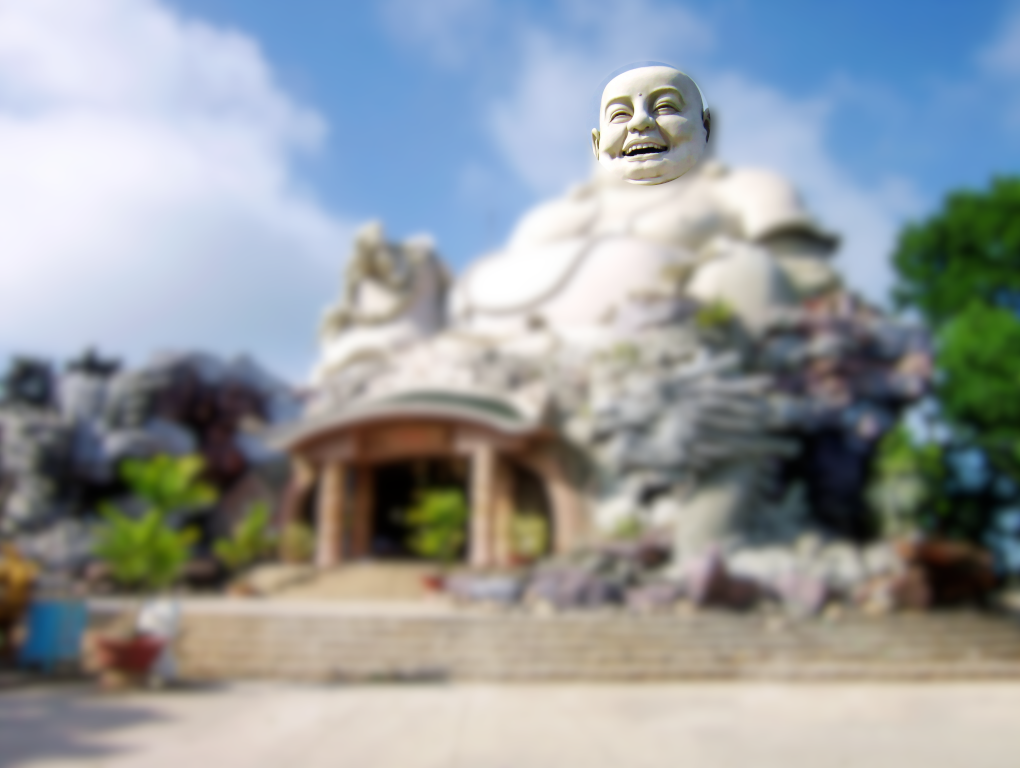
\includegraphics[width=\textwidth,height=\textheight,keepaspectratio]{logos/FoveatedImage.png}
     \caption{Foveated Rendered Image, picture originally from the DIVK dataset \parencite{Agustsson2017}.}
    \label{fig:foveated-rendering}
\end{figure*}

\par
One method to tackle the problem with the necessary quality level is to use foveated rendering. Initially, foveated rendering is used in the gaming area to increase quality while keeping high frames per second, and without it there would be curtailments in quality or FPS. The foveated rendering simulates the human’s view which is separated into two regions. The first is the foveal region, which is approximately 5$^{\circ}$ of the visual sight, is in the centre of the current gaze and is responsible for a sharp view \parencite{Yanoff2020}. The remaining view is grouped to the peripheral region and is less sharp and clear compared to the foveal region \parencite{Yanoff2020}. This fact leads to computing an image which has high resolution and full details at the current gaze while the background displays only contours of objects and is blurry. For example, see \autoref{fig:foveated-rendering} in which the head of the buddha statue is sharp, and the rest becomes blurrier. One requirement for this method is that the gaze’s current location can be determined in the image, which requires modern \gls{vr} glasses like the HTC VIVE Pro Eye \parencite{HTCVIVEProEye2020} or additional separate hardware like the Tobii Eye Tracker \parencite{TobiiTracker2020}. For streaming, foveated renering reduces the needed bandwidth while keeping good quality and reducing the latency.
\par
Another method for solving the streaming problem is to use \gls{ml}. With the increase of available hardware power, \gls{ml} is becoming more available for developers and users through consumer hardware. For streaming, the compression and decompression data are necessary steps and are typical for autoencoders. The problem with autoencoders is that they learn how to compress and decompress detailed data, and the outcome is restricted to this (training) material, whereas it needs to work with any unknown data. A different approach is to increase the quality of images after the transmission. For enhancing the quality of videos or images, \gls{sr} is a promising method as it is a set of methods that reduce image noise and deblur. One of the newest and most suitable working methods is a \gls{gan} which is a deep convolutional neural network. Developed in 2014 by \citeauthor{Goodfellow2014}, \gls{gan} was first used to generate new images from random noise, for example handwritten numbers. Later on, it developed to a promising \gls{sr} method, with a low-resolution input and a high-resolution output. A prominent example is the \gls{srgan}, which is capable of generating realistic single textures \parencite{Ledig2017}. With DeepFovea, Facebook’s research lab tackled the problem of enhancing video sequences with \gls{gan} \parencite{Kaplanyan2019}. The original idea of DeepFovea was to enhance foveated rendered videos for \gls{vr} and to reduce the needed hardware power by reducing the resolution and restoring the background while keeping the foveal area in original high-density resolution.
\par
In conclusion, a stable streaming solution is required for telepresence that delivers a high-resolution video within a limited latency independently of the network conditions. The goal of this thesis is to build a streaming solution of 3D video data from one computer to another. On the receiver side, a \gls{hmd} is connected and displays the environment of the robot. The following steps were implemented: On the robot’s side called server, a camera is attached to record the environment. The camera stream is split into two parts. The first one is a high-resolution uncompressed video of the foveal area and the second one is a low-resolution compressed video of the peripheral area. For generating the foveal area, the server receives the current gaze of the user sequentially from the client. After both images are generated, and the peripheral region got compressed based on the available bandwidth, they are transmitted to the client. The client, where the \gls{hmd} is connected to, receives both streams and merges them according to the prior sent gaze coordinates. If necessary, the client performs SR of the peripheral region to achieve an overall good video quality. The resulting image is displayed in VR. For the next image, the client sends the \glspl{hmd} current predicted gaze to the server. The maximum latency from the robot to the user should be below 125 milliseconds.
\par
In order to achieve this goal, \autoref{chapter:background} introduces the current state of the art and the background of the used technologies to get a better understanding of the implementation. For a better comparison of the measuring, between different applications, \autoref{chapter:environment} introduces the used hard- and software. Chapter \ref{chapter:implementation} describes the implementation of low-latency streaming with foveated rendering and superresolution. The measured results of the formerly described implementation are presented in \autoref{chapter:evaluation}. Last but not least, \autoref{chapter:conclusion} outlines the conclusion and identifies the limitations. Finally, \autoref{chapter:outlook} gives a brief outlook for the next steps.